\chapter*{符號列表}
\label{chp:symbol}
% \addcontentsline{toc}{chapter}{符號列表}


%英文字母 -> 希臘字母%
%小寫 -> 大寫%
%向量 -> 純量% %粗->細%


\section*{符號列表}
\subsection*{座標系}

\begin{longtable}[l]{cl}
    % $\text{Bell}(\cdot)$ & 鐘形函式\\
    $P$ & 座標點\\
    $x,y,z$ & 座標點$P$的$x,y,z$分量\\
    $N$ & 單位向量\\
    $u,v,w$ & 單位向量$N$的$x,y,z$分量\\
    $\alpha$ & 球座標系中的仰角分量\\
    $\beta$ & 球座標系中的方位角分量\\
\end{longtable}

% \begin{figure}[ht]
% 	\centering
% 	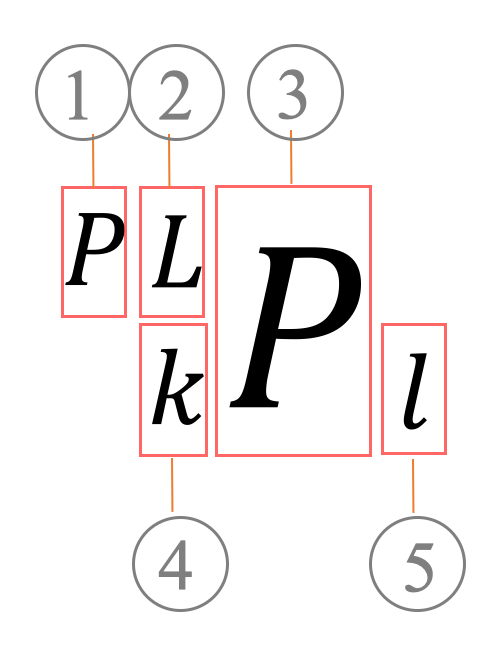
\includegraphics[width=3cm]{ch1pic/not_pos.png}
%     \caption{座標系小標解釋}
%     \label{pic:not_pos}
% \end{figure}

% \begin{description}
%     \item[(1)] 投影至的座標系($P$: PD座標系;$L$: LED座標系)
%     \item[(2)] 定義於哪個座標系($P$: PD座標系;$L$: LED座標系)
%     \item[(3)] 座標系符號(如上表)
%     \item[(4)] 第$k$個樣本點($k=1,2,...,K$)
%     \item[(5)] 第$l$個LED或第$p$個PD($l=1,2,...,L$;$p=1,2,...,P$)
% \end{description}



\onehalfspacing

\subsection*{座標系轉換}

\begin{longtable}[l]{cl}
    $\boldsymbol{H}$ & 齊次轉換矩陣 Homogeneous Transformation Matrix\\
    $\boldsymbol{T}$ & 平移向量 Transfer Vector\\
    $\boldsymbol{Ro}$ & 旋轉矩陣 Rotation Matrix\\
\end{longtable}

% \begin{figure}[ht]
% 	\centering
% 	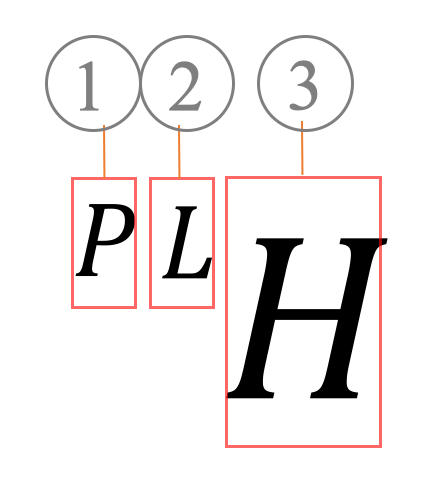
\includegraphics[width=3cm]{ch1pic/not_transform.png}
%     \caption{座標系轉換小標解釋}
%     \label{pic:not_transform}
% \end{figure}

% \begin{description}
%     \item[(1)] 投影至的座標系($P$: PD座標系;$L$: LED座標系)
%     \item[(2)] 定義於哪個座標系($P$: PD座標系;$L$: LED座標系)
%     \item[(3)] 座標系轉換符號(如上表)
%     \item[(4)] 第$k$個樣本點($k=1,2,...,K$)] 
% \end{description}


\onehalfspacing

\subsection*{LED與PD的交互關係}

\begin{longtable}[l]{cl}
    % $\text{Bell}(\cdot)$ & 鐘形函式\\
    $\phi$ & PD入射角\\
    $\theta$ & LED出射角\\
    $D$&距離\\
\end{longtable}

% \begin{figure}[ht]
% 	\centering
% 	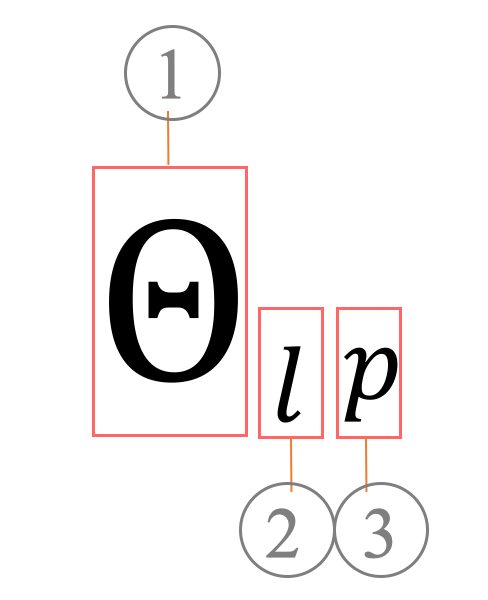
\includegraphics[width=3cm]{ch1pic/not_interactive.png}
%     \caption{LED與PD的交互關係小標解釋}
%     \label{pic:not_interactive}
% \end{figure}

% \begin{description}
%     \item[(1)] LED與PD的交互關係符號(如上表)
%     \item[(2)] 第$l$個LED($l=1,2,...,L$)
%     \item[(3)] 第$p$個PD($p=1,2,...,P$)
%     \item[(4)] 第$k$個樣本點($k=1,2,...,K$) 
% \end{description}

\onehalfspacing

\subsection*{硬體參數}

\begin{longtable}[l]{cl}
    % $\text{Bell}(\cdot)$ & 鐘形函式\\
    符號 & LED硬體參數\\ \hline
    $M$ & LED的朗伯次方(Lambertian Order)\\
    $Pt$ & 總輻射通量(Total Radiation Flux) 
\end{longtable}

\begin{longtable}[l]{cl}
    % $\text{Bell}(\cdot)$ & 鐘形函式\\
    符號 & PD硬體參數\\ \hline
    $m$ & PD的朗伯次方(Lambertian Order)\\
    $A$ & 有效面積\\
    $Re$ & 響應率(Responsivity)\\
\end{longtable}


\onehalfspacing

\subsection*{光學領域單位}

\begin{longtable}[l]{cllll}
    % $\text{Bell}(\cdot)$ & 鐘形函式\\
    符號& 中文& 英文 & 單位符號&國際單位制\\\hline
    $\Omega$ & 立體角&Solid Angle& $sr$&球面度(Steradian) \\
    $\omega$ & 角度&Angle& $rad$&弧度(radian)\\
    $r$ & 半徑&Radius&  $m$ &公尺\\
    $\Phi$ & 輻射通量&Radiation Flux& $W$&瓦特(Watt)\\
    $I$ & 輻射強度&Radiation Intensity & $W\cdot sr^{-1}$&瓦特每球面度 \\
    $E$ & 輻照度&Irradiance&$W\cdot m^{-2}$ &瓦特每平方公尺\\
\end{longtable}




\onehalfspacing

\section*{小標解釋}

論文中由於座標系、硬體數量、樣本數量眾多,為了區分不同上下小標的意義,以圖\ref{pic:symbol}呈現各小標意思,左上標表示座標系,左下標顯示是哪個樣本,而右下標則依照物理量代表著LED或PD的編號,在LED與PD交互關係的物理量中右下標同時包含兩者的編號。

\begin{figure}[ht]
    \caption{符號小標解釋}
    \label{pic:symbol}
	\centering
	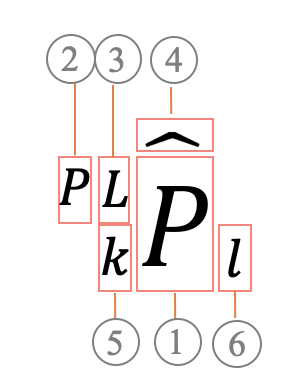
\includegraphics[width=3cm]{ch1pic/not_whole.png}
\end{figure}



\begin{description}
    \item[(1)] 符號
    \item[(2)] 投影至的座標系($P$: PD座標系;$L$: LED座標系)
    \item[(3)] 定義於哪個座標系($P$: PD座標系;$L$: LED座標系)
    \item[(4)] $\hat{(\cdot)}$代表該物理量為量測所得或處理量測所得訊號而得
    \item[(5)] 第$k$個樣本點($k=1,2,...,K$)
    \item[(6)] 第$p$個PD($p=1,2,...,P$)或第$l$個LED($l=1,2,...,L$);LED與PD交互關係物理量的(6)小標為$lp$兩者的交互關係
\end{description}